%!TEX root = ../rapport.tex
%!TEX encoding = UTF-8 Unicode

% Chapitres "Introduction"

% modifié par Francis Valois, Université Laval
% 31/01/2011 - version 1.0 - Création du document


\label{s:experimentation}
\chapter{Laboratoire 5}
\section{Projet 1: Mesure de longueur}
La ligne que nous cherchons à mesurer est une combinaison de deux lignes de 6m de câble de RG59. La démarche que nous employons est la suivante:
\begin{enumerate}
\item Insérer un court-circuit comme charge en fin de ligne;
\item Localiser la fréquence pour laquelle la tension est maximale;
\item Localiser la fréquence pour laquelle la tension est minimale;
\item Utiliser l'équation : $ l = \frac{v_p}{4\left|f_{cc} - f_{co}\right|}$
\end{enumerate}
Nous avons choisi cette démarche en sachant que l'équation présentée dans notre démarche permet de localiser un court-circuit sur une ligne. Ce faisant, on obtient directement la distance par rapport à la source, tel que désiré. Les données obtenues sont les suivantes:
\begin{itemize}
\item $f_{co} = 4.05MHz $
\item $f_{cc} = 9MHz$
\end{itemize}
On obtient alors:
\begin{equation}
l = \frac{v_p}{4\left|f_{cc} - f_{co}\right|} = \frac{0.66\cdot c}{4\times 10^6\left|9 - 4.05\right|} = 10m
\end{equation}
\section{Projet 2: Effet des charges sur les signaux à l'entrée}
Les résultats obtenus pour l'expérience sur la variation de fréquence pour caractériser la localisation des min et des max en courant et en tension sont présentés dans les tableaux \ref{tab:1} et \ref{tab:2}. Les données recueillies sont des valeurs crête à crête. 
\begin{table}[htbp]
  \centering
    \begin{tabular}{|c|c|c|c|c|}\hline
    Fréquence & $V_{min}$ & $V_{max}$ & $I_{min}$ & $I_{max}$ \\\hline
    MHz   & mV    & mV    & mA    & mA \\\hline
    0.3   &       & 3040  & 8.8    &  \\
    4.377 & 220   &       &       & 40.8 \\
    9.017 &       & 2940  & 4.4    &  \\
    13.407 & 240   &       &       &  \\
    13.507 &       &       &       & 46.0 \\
    17.217 &       & 2900  &       &  \\
    18.097 &       &       & 4.4    &  \\\hline
    \end{tabular}%
      \caption{Résultats obtenus pour un circuit ouvert en fin de ligne}
  \label{tab:1}%
\end{table}%

\begin{table}[htbp]
  \centering
    \begin{tabular}{|c|c|c|c|c|}\hline
    Fréquence & $V_{min}$ & $V_{max}$ & $I_{min}$ & $I_{max}$ \\\hline
    MHz   & mV    & mV    & mA    & mA \\\hline
          &       &       &       &  \\
    4.1   &       &       & 14.8   &  \\
    4.3   &       & 2.26  &       &  \\
    8.93  & 940   &       &       &  \\
    8.73  &       &       &       & 34.0 \\
    12.89 &       & 2.22  &       &  \\
    13.07 &       &       & 16.6   &  \\
    17.74 & 960   &       &       &  \\
    17.87 &       &       &       & 40.0 \\\hline
    \end{tabular}%
  \caption{Résultats obtenus pour un charge de 27$\Omega$ en fin de ligne}
  \label{tab:2}%
\end{table}%

\subsection{Calcul de $Z_0$}
Il est demandé d'identifier expérimentalement, au moyen du circuit ouvert, l'impédance caractéristique de la ligne $Z_0$. On sait premièrement que:

\begin{equation}
V^+ = \frac{V_{max} + V_{min}}{2}
\end{equation}
On sait aussi que l'impédance caractéristique est donnée par:
\begin{equation}
Z_0 = 2\frac{V^+}{I_{max} + I_{min}}
\end{equation}

En substituant:

\begin{equation}
Z_0 = \frac{V_{max} + V_{min}}{I_{max} + I_{min}}
\end{equation}


Selon le tableau \ref{tab:1}, on a que $V_{max}$ est de 2.96 V, que $V_{min}$ est de 0.23 V, que $I_{max}$ est de 0.0434 A et que $I_{min}$ est de 0.0059 A. On trouve finalement $Z_0 = 64.71 \Omega $. La valeur théorique du câble employé est de $73\Omega$, on remarque un écart relativement important  (11\%) entre ce qui était attendu et ce qui fut obtenu. Le manque de stabilité des mesures à l'oscilloscope dans les plages inférieures permet de justifier pourquoi il est difficile d'obtenir des valeurs fiables. D'autant plus que les valeurs des extremums n'étaient pas exactement aux mêmes endroits en courant et en tension.

\subsection{Calcul du SWR}
Il existe deux manières de calculer le SWR, soit au moyen du courant et au moyen de la tension. Afin de déterminer le SWR, on applique le développement suivant:
\begin{equation}
SWR = \frac{V_{max}}{V_{min}} = \frac{I_{max}}{I_{min}}
\end{equation}

On utilise les valeurs moyennes de chacuns des paramètres obtenus lors des manipulations expérimentales, ces valeurs sont présentées au tableau \ref{tab:2}.
\begin{equation}
SWR = \frac{V_{max}}{V_{min}} = \frac{2.24}{0.95} = 2.358
\end{equation}
\begin{equation}
SWR = \frac{I_{max}}{I_{min}} = \frac{37}{15.7} = 2.357
\end{equation}

On remarque que les deux méthodes de calcul convergent vers le même résultat.

\section{Projet 3: Comportement en fréquence à l'entrée et au milieu avec court-circuit}
Les multiples données sont présentées au tableau \ref{tab:3}. Afin d'alléger la présentation, la notation : $\Delta \Phi$ a été employée pour désigner le déphasage. Le déphasage mesuré à l'oscilloscope est présenté en nanosecondes, tandis que le déphasage ramené à la fréquence est présenté en radians. Ces données nous permettent de tracer des comparaisons avec la théorie. 

\paragraph{} La tension en fonction de la fréquence pour une distance $d = \frac{l}{2}$ a été tracée d'une part selon les données obtenues expérimentalement et d'autre part, au moyen de l'allure théorique des courbes. Le résultat de ce tracé est présenté à la figure \ref{fig:1}. Comparée à la courbe théorique, la courbe expérimentale présente une atténuation moins rapide dans la partie gauche (inférieure à $\frac{\lambda}{2}$). Par ailleurs, la position du minimum de tension de la courbe expérimentale est en avance de 500kHz sur celui de la courbe théorique. Aussi, le minimum de la courbe expérimentale est de 200mV supérieur à celui de la courbe théorique. Le comportement des deux courbes est similaire dans la portion de fréquence supérieure à 10MHz. On peut conclure des suppositions théoriques et confirmer la validité du modèle étudié pour ce cas selon la similitude dans la forme des courbes obtenues.

\paragraph{}La tension en fonction de la fréquence pour une distance $d = l$ a été tracée d'une part selon les données obtenues expérimentalement et d'autre part, au moyen de l'allure théorique des courbes. Le résultat de ce tracé est présenté à la figure \ref{fig:2}.Par rapport à la courbe théorique, la courbe expérimentale est en avance d'environ 500kHz. L'amplitude du minimum est de 200mV par rapport à  celui de la courbe théorique qui avoisine les 50mV. On remarque la présence d'un maximum vers 10MHz dont l'amplitude expérimentale est de 2840mV par rapport à une amplitude théorique de 3100mV. On peut associer ce décalage d'amplitude aux pertes (négligées dans le modèle) de la ligne. Le comportement des deux courbes est similaire sur l'ensemble de la plage de fréquence tracée. On peut conclure des suppositions théoriques et confirmer la validité du modèle étudié pour ce cas selon la similitude dans la forme et des valeurs dans les courbes obtenues.

\paragraph{}Le courant en fonction de la fréquence pour une distance $d = l$ a été tracée d'une part selon les données obtenues expérimentalement et d'autre part, au moyen de l'allure théorique des courbes. Le résultat de ce tracé est présenté à la figure \ref{fig:3}.Par rapport à la courbe théorique, la courbe expérimentale est en avance d'environ 500kHz. On remarque la localisation d'un maximum vers 5MHz. Les amplitudes sont pratiquement égales (si l'on tient compte des décalages) $\Delta I \approx 1\mu A$. On remarque la présence d'un minimum vers 10MHz dont l'amplitude expérimentale est de 5,2mA par rapport à  celui de la courbe théorique qui est de 1.35mA. Le comportement des deux courbes est similaire sur l'ensemble de la plage de fréquence tracée. On peut conclure des suppositions théoriques et confirmer la validité du modèle étudié pour ce cas selon la similitude dans la forme et des valeurs dans les courbes obtenues.

\paragraph{}Le déphasage en fonction de la fréquence pour une distance $d = l$ a été tracée d'une part selon les données obtenues expérimentalement et d'autre part, au moyen de l'allure théorique des courbes. Le résultat de ce tracé est présenté à la figure \ref{fig:4}.Par rapport à la courbe théorique, la courbe expérimentale présente des montées avec des transitions moins brusques que pour la courbe théorique. Ce qui est normal vu les limititations expérimentales dans la mesure des transitions brusques. On remarque la localisation d'un plateau déphasé de $-\frac{\pi}{2}$ de 0 à 5MHz ainsi que de 10MHz à 15Mhz. L'amplitude moyenne de ces plateaux expérimentaux est inférieure de 0.2 rad à celle du plateau théorique. Aussi un plateau est présent de 5MHz à 10MHz, l'amplitude moyenne de celui-ci est de 0.4 rad inférieure à celle de la courbe théorique. Si l'on reporte ces résultats à la théorie, on peut valider le fait que les signaux subissent un décalage de 180$^\circ$ lors des passages par les multiples entiers de $\frac{\lambda}{4}$. Dans un cas, la tension est en avance sur le courant et dans l'autre, le courant est en avance sur la tension. On peut conclure des suppositions théoriques et confirmer la validité du modèle étudié pour ce cas selon la similitude dans la forme et des valeurs dans les courbes obtenues.

\begin{table}[H]
  \centering
    \begin{tabular}{|c|c|c|c|c|c|}\hline
    Fréquence & $V\left(\frac{l}{2}\right)$ & $V(l)$ & $I(l)$ & $\Delta \Phi (s)$ & $\Delta \Phi (rad)$ \\\hline
    MHz   & mV    & mV    & mA    & ns    & rad \\\hline
    0.5   & 2940  & 2900  & 15.2  & -520  & -1.6 \\
    1.0   & 2740  & 2600  & 22.4  & -240  & -1.5 \\
    1.5   & 2480  & 2200  & 28.4  & -170  & -1.6 \\
    2.0   & 2220  & 1800  & 33.6  & -140  & -1.8 \\
    2.5   & 2000  & 1400  & 35.6  & -108  & -1.7 \\
    3.0   & 1800  & 1000  & 38.4  & -90   & -1.7 \\
    3.5   & 1640  & 680   & 40    & -76   & -1.7 \\
    4.0   & 1500  & 340   & 40.8  & -58   & -1.5 \\
    4.5   & 1400  & 200   & 42.4  & 10    & 0.3 \\
    5.0   & 1300  & 440   & 42    & 38    & 1.2 \\
    5.5   & 1200  & 760   & 38.4  & 35    & 1.2 \\
    6.0   & 1120  & 1060  & 37.2  & 30    & 1.1 \\
    6.5   & 1000  & 1380  & 37.2  & 27    & 1.1 \\
    7.0   & 920   & 1720  & 35.2  & 26    & 1.1 \\
    7.5   & 800   & 2080  & 32    & 23    & 1.1 \\
    8.0   & 680   & 2400  & 27.6  & 23    & 1.2 \\
    8.5   & 540   & 2660  & 21.6  & 20    & 1.1 \\
    9.0   & 340   & 2840  & 12.4  & 16    & 0.9 \\
    9.5   & 160   & 2800  & 5.2   & -2    & -0.1 \\
    10.0  & 280   & 2680  & 11.2  & -25   & -1.6 \\
    10.5  & 500   & 2400  & 19.2  & -27   & -1.8 \\
    11.0  & 720   & 2080  & 27.2  & -26   & -1.8 \\
    11.5  & 940   & 1640  & 32.4  & -26   & -1.9 \\
    12.0  & 1160  & 1260  & 37.2  & -24   & -1.8 \\
    12.5  & 1320  & 860   & 41.2  & -22   & -1.7 \\
    13.0  & 1500  & 500   & 43.6  & -18   & -1.5 \\
    13.5  & 1760  & 252   & 46    & -2    & -0.2 \\
    14.0  & 2000  & 630   & 46    & 6     & 0.5 \\\hline
    
    \end{tabular}%
 \caption{Tableau présentant les données obtenues lors de l'analyse du comportement en fréquence à l'entrée et au milieu avec un circuit ouvert}
 \label{tab:3}%
 \end{table}%
 \begin{figure}[H]
\centering
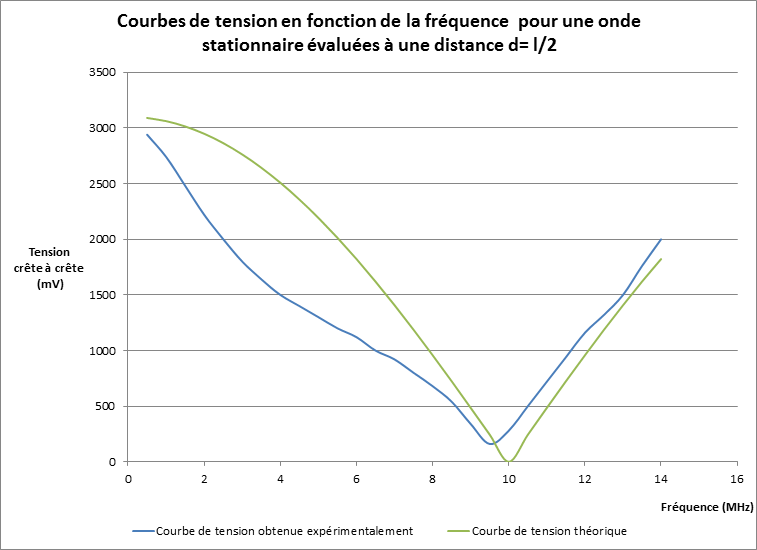
\includegraphics[scale=0.45]{question31.png}
\caption{Figure présentant la comparaison des courbes de tension (mV) en fonction de la fréquence (MHz) d'une onde stationnaire pour une distance $d = l$ obtenues expérimentalement et théoriquement}
\label{fig:1}
\end{figure}
\begin{figure}[H]
\centering
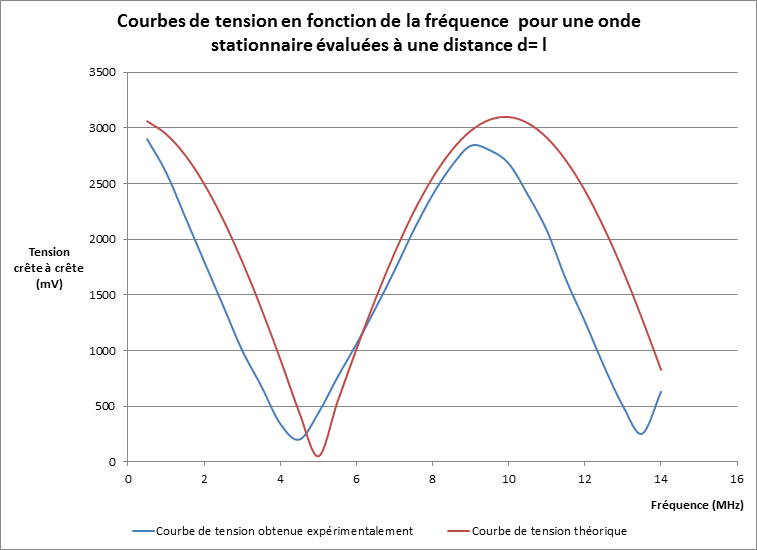
\includegraphics[scale=0.45]{question32.png}
\caption{Figure présentant la comparaison des courbes de tension (mV) en fonction de la fréquence (MHz) d'une onde stationnaire pour une distance $d = l$ obtenues expérimentalement et théoriquement}
\label{fig:2}
\end{figure}
\begin{figure}[htbp]
\centering
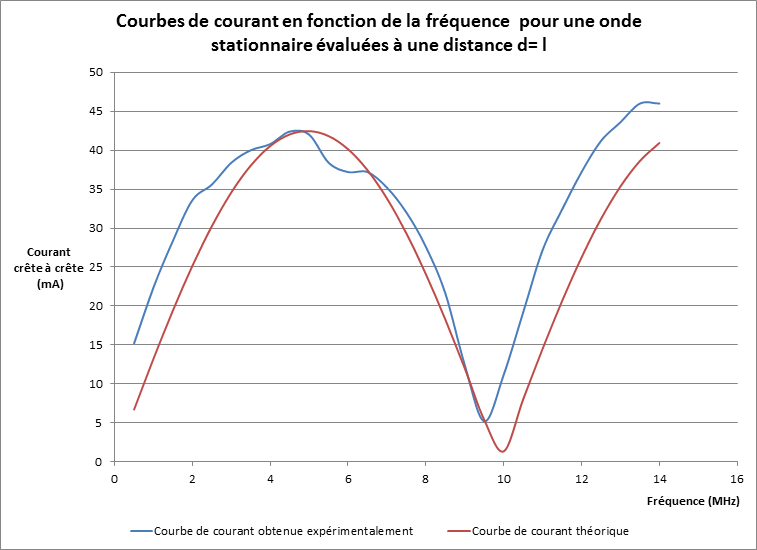
\includegraphics[scale=0.45]{question33.png}
\caption{Figure présentant la comparaison des courbes de courant (mA) en fonction de la fréquence (MHz) d'une onde stationnaire pour une distance $d = l$ obtenues expérimentalement et théoriquement}
\label{fig:3}
\end{figure}
 \begin{figure}[H]
\centering
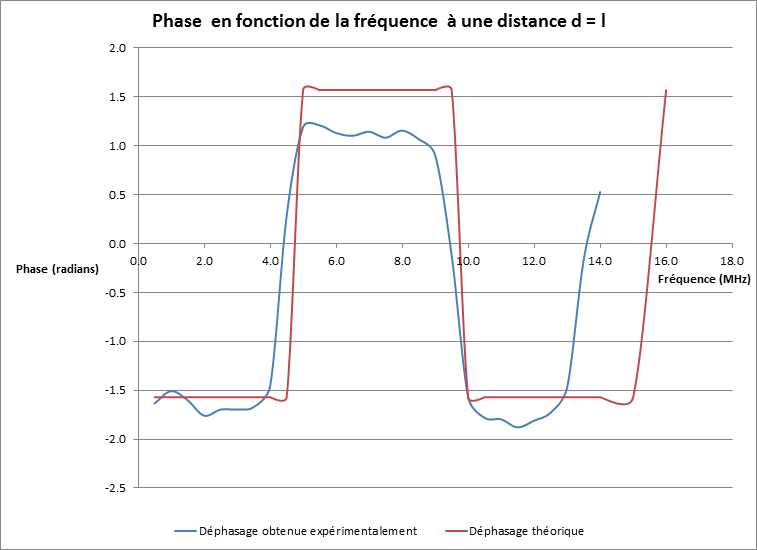
\includegraphics[scale=0.45]{question34.png}
\caption{Figure présentant la comparaison des courbes de déphsage (radians) en fonction de la fréquence (MHz) d'une onde stationnaire pour une distance $d = l$ obtenues expérimentalement et théoriquement}
\label{fig:4}
\end{figure}
  
